\subsection{Text-Based Retrieval-Augmented Generation}
\subsubsection{Retrieval-Augmented Generation}

Early research on document-level question answering (DocQA) faced two core challenges: first, Large Language Models (LLMs) were limited by context length, making it difficult to directly process long or multi-document inputs; second, pure generative models were prone to hallucinations when lacking external evidence constraints, performing unstably in fact-dense scenarios or those requiring cross-document reasoning. Against this backdrop, researchers initially proposed the Retrieval-Augmented Generation (RAG) paradigm, which combines information retrieval with text generation. Its core intuition was to first retrieve evidence relevant to the question from an external document collection and then guide the language model to generate an answer within a controlled context, thereby enhancing factual coverage and answer reliability without significantly increasing the model size. Early RAG primarily followed the classic "retrieve-then-generate" paradigm, which improved DocQA performance by enhancing evidence recall quality and multi-hop support capabilities. Triple-Fact Retriever \cite{wu2022triple} improved the accuracy and interpretability of cross-document evidence paths in multi-hop DocQA by extracting structured triple facts and aggregating evidence hop by hop. Multi-Document Question Answering with Lightweight Embeddings-based Document Reranker \cite{aitymbetov2024multi} employed a two-stage retrieval process combining BM25 coarse-ranking with lightweight embedding-based re-ranking, improving evidence quality in multi-document QA while maintaining efficiency. Zero-Shot Complex Question-Answering on Long Scientific Documents \cite{wang2025zero} integrated RAG with question decomposition, multi-hop reasoning, and long-answer generation, achieving complex QA on long documents without task-specific fine-tuning. Meanwhile, DR-RAG \cite{hei2024dr} mitigated evidence omission in multi-hop QA caused by static similarity retrieval by introducing dynamic document relevance modeling and a two-stage filtering mechanism.

Building on traditional RAG improvements centered on retrieval quality and multi-hop support, subsequent research began to focus further on utilizing the reasoning capabilities of LLMs and internal or cross-document structural information to construct more structure-aware and reasoning-guided retrieval-augmentation frameworks. Among these, DocReLM: Mastering Document Retrieval with Language Model \cite{wei2024docrelm} fine-tuned retrievers and re-rankers by introducing LLMs to generate domain-specific training data and utilized LLM-generated citation networks to expand candidate document sets, thereby significantly enhancing semantic understanding and cross-literature association discovery in academic literature retrieval. Advanced Chain-of-Thought Reasoning for Parameter Extraction from Documents Using Large Language Models \cite{chen2025advanced} introduced an improved chain-of-thought reasoning mechanism into document-level information extraction tasks, achieving reasoning-driven refined retrieval and parameter localization through modules such as Targeted Document Retrieval, Iterative Retrieval Optimization, and Preference Optimization. Semi-Structured Chain-of-Thought: Integrating Multiple Sources of Knowledge for Improved Language Model Reasoning \cite{su2024semi} further explored the unification of parametric knowledge, structured knowledge graphs, and unstructured text retrieval into a semi-structured reasoning chain, allowing multi-source knowledge to be progressively filled and integrated during the reasoning process. In long-document scenarios, Beyond Chunking: Discourse-Aware Hierarchical Retrieval for Long Document Question Answering \cite{chen2025chunkingdiscourseawarehierarchicalretrieval} utilized Rhetorical Structure Theory (RST) for discourse-level modeling of documents and performed hierarchical retrieval on this structure, effectively alleviating the issue of semantic incoherence caused by flat chunking. For multi-document scenarios, Knowledge Graph Prompting for Multi-Document Question Answering \cite{wang2024knowledge} enhanced global consistency and multi-document reasoning capabilities by constructing cross-document knowledge graphs and guiding the LLM through graph-traversal evidence collection. Meanwhile, PdfTriage: Question Answering over Long, Structured Documents \cite{saad2024pdftriage} focused on structured long-document QA, explicitly modeling structural meta-information such as pages, sections, and tables to enable RAG to accurately respond to queries containing structural references. Overall, work in this stage marked the evolution of RAG from "similarity-centric retrieval augmentation" to a "document-level information acquisition paradigm driven jointly by structure and reasoning."

Despite the significant improvements in evidence localization and multi-document understanding achieved by the aforementioned works through document structure, knowledge graphs, and reasoning-guided retrieval, their overall processes still largely relied on preset retrieval strategies. The connection between retrieval and reasoning was often a "retrieve-then-reason" sequence, making it difficult to dynamically adjust retrieval paths, depth, and evidence combinations as reasoning unfolds. In long-document, multi-hop, and multi-document QA scenarios, this static retrieval mode still readily resulted in broken evidence chains, accumulation of redundant information, or omission of critical evidence. To address this, subsequent RAG research further treated "retrieval" as a decision-making step directly driven and scheduled by the reasoning process: First, From Local to Global: A Graph RAG Approach to Query-Focused Summarization \cite{edge2024graphrag} (GraphRAG) proposed a graph-enhanced retrieval framework based on knowledge graphs and community detection, achieving precise understanding and comprehensive answers for global, cross-document queries by constructing entity-relationship graphs and generating hierarchical community summaries. Subsequently, LightRAG: Simple and Fast Retrieval-Augmented Generation \cite{guo2024lightrag} addressed the high computational overhead of GraphRAG by designing a lightweight dual-level index architecture, significantly reducing indexing time and storage costs while retaining the semantic advantages of graph structures, thus enhancing reasoning efficiency and facilitating the industrial deployment of graph-enhanced RAG. Furthermore, HyperGraphRAG: Retrieval-Augmented Generation via Hypergraph-Structured Knowledge Representation \cite{he2024hypergraphrag} broke through the theoretical limitations of traditional binary graphs by introducing hypergraph structures to directly model n-ary relations, preserving the semantic integrity of complex events by connecting multiple entities through a single hyperedge, thus achieving more accurate knowledge retrieval and generation in scenarios highly dependent on n-ary relationship reasoning, such as medical and legal fields. Leveraging Spreading Activation for Improved Document Retrieval in Knowledge-Graph-Based RAG Systems \cite{pavlovic2025leveraging} enabled activation values to propagate dynamically along evidence chains for prioritized retrieval of relevant fragments by automatically constructing knowledge graphs and executing spreading activation, serving as a plug-and-play module that enhanced multi-hop evidence continuity in chain-based reasoning. GARLIC: LLM-Guided Dynamic Progress Control with Hierarchical Weighted Graph for Long Document QA \cite{wang2024garlic} constructed a hierarchical weighted directed acyclic graph based on LLM attention for dynamic retrieval, allowing retrieval paths and information volume to be adaptively controlled by the LLM, overcoming the limitations of traditional vector similarity and fixed tree summarization. For multi-document environments, HiQA: A Hierarchical Contextual Augmentation RAG for Multi-Documents QA \cite{chen2024hiqa} transformed documents into hierarchical structures with cascading metadata and fused vector, BM25, and keyword matching through multi-path retrieval to improve retrieval discriminability in structurally similar document sets. For complex hierarchical documents, BookRAG: A Hierarchical Structure-aware Index-based Approach for Retrieval-Augmented Generation on Complex Documents \cite{wang2025bookrag} built BookIndex, fusing logical hierarchy trees and entity-relationship graphs, and introduced an agentic retrieval strategy inspired by information foraging theory to dynamically select retrieval workflows, thereby balancing recall, efficiency, and multi-hop path integrity. In multi-hop reasoning, Enhancing Document-Level Question Answering via Multi-Hop Retrieval-Augmented Generation with LLaMA 3 \cite{huang2025enhancing} integrated dense retrieval, context fusion, and multi-hop mechanisms, strengthening retrieval-generation synergy through the joint optimization of retrieval likelihood and generation loss. Finally, Chain of Retrieval: Multi-Aspect Iterative Search Expansion and Post-Order Search Aggregation for Full Paper Retrieval \cite{park2025chain} drove iterative expansion retrieval via multi-aspect decomposition and reorganized hierarchical evidence through post-order aggregation, reflecting a paradigm shift in which the retrieval process itself served as the reasoning chain. Overall, work in this stage marked the further evolution of RAG from "structure-aware retrieval augmentation" to a modular retrieval and generation framework dynamically driven by the reasoning process.

\begin{figure*}[t]
\centering
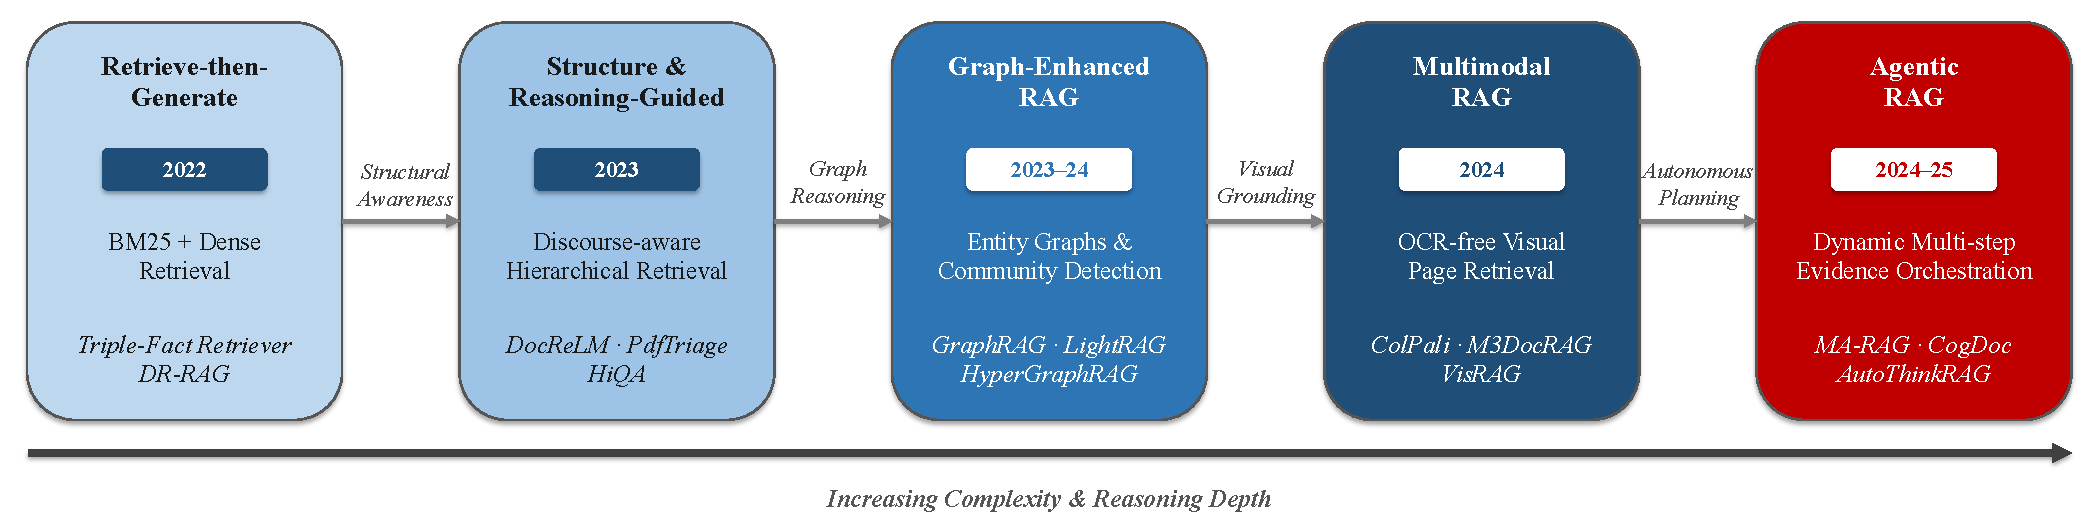
\includegraphics[
    width=0.95\textwidth,
    height=0.38\textheight,
    keepaspectratio,
    trim=0cm 0cm 0cm 0cm,
    clip
]{figs_by_qixingyu/fig06.pdf}
\caption{Five-stage evolution of retrieval-augmented generation paradigms for document question answering, progressing from Retrieve-then-Generate (2022) through Structure and Reasoning-Guided RAG (2023), Graph-Enhanced RAG (2023--2024), Multimodal RAG (2024), and Agentic RAG (2024--2025), with representative systems listed at each stage and increasing complexity and reasoning depth indicated along the horizontal axis.}
\label{fig:rag_evolution}
\end{figure*}

\subsubsection{End-to-End Document Question Answering}

\paragraph{Early Attention Mechanisms}
Document understanding originated with the construction of attention mechanisms to capture context. Dynamic Coattention Networks \cite{dynamiccoattention2017} proposed a co-attention strategy to capture bidirectional interaction information by simultaneously attending to the question and the document. Addressing the excessive search range in long documents, Coarse-to-fine question answering \cite{coarsetofine2017} pioneered a "coarse-to-fine" two-stage framework: first retrieving relevant sentences, then extracting precise answers. To further enhance text representation capabilities, EA Reader \cite{eareader2019} utilized multi-space context fusion to improve performance in cloze-style QA.

\paragraph{Reasoning Based on Graph Structures and Global Information}
As document length and complexity continued to increase, Graph Neural Networks (GNNs) became the core paradigm for connecting discrete pieces of evidence. Question Answering by Reasoning Across Documents with GCNs \cite{gcnmultihop2019} was among the earliest works to utilize entity-based Graph Convolutional Networks for handling multi-hop tasks. Subsequently, Identifying Supporting Facts with Document Graph Networks \cite{dgn2019} further shifted the research focus from answer prediction to the explicit identification of supporting facts. This shift was achieved by modeling multi-document contexts as sentence-level document graphs and introducing question-conditioned GNN reasoning mechanisms on the graph structure. Meanwhile, the Heterogeneous Graph approach \cite{heterograph2019} handled cross-document reasoning by modeling different types of nodes (e.g., entities, documents). In recent research, Path-based GCN \cite{pathgcn2020} emphasized reasoning along specific relational paths, while Capturing global structural information in long document question answering with compressive graph selector network \cite{cgsn2022} achieved more efficient long-document QA through integrated global structural encoding.

To improve the capability and interpretability of multi-hop QA, researchers began exploring explicit reasoning chains and explainable frameworks. First, Exploiting Explicit Paths \cite{explicitpaths2019} proposed that the key lay in selecting a correct evidence path, with the model scoring and choosing within a path space. Multi-hop Question Answering via Reasoning Chains \cite{reasoningchains2020} proposed the use of "reasoning chains" as intermediate explicit variables, where the model predicted one or more reasoning chains before generating an answer. Explore, Propose, and Assemble \cite{epa2019} proposed a three-stage explainable reasoning framework to bridge information fragments. Further progress in explainability included Select, Answer and Explain \cite{sae2020}, which simultaneously generated answers and evidence rationales, elevating "explanation" from an auxiliary task to an output as important as the answer itself. Hop, Union, Generate \cite{hug2023} proposed guiding the model to form an explainable reasoning process without explicit evidence supervision. Additionally, Ask to Understand \cite{asktounderstand2023} proposed revealing complex multi-hop logic clearly by generating a series of intermediate questions.

\paragraph{Task Generalization and the LLM Era}
Methods such as multi-hop reasoning expanded from pure QA to broader document-level tasks. Multi-Hop Transformer \cite{multihoptransformer2021} explicitly introduced multi-hop reasoning into the translation field for the first time. Syntax-enhanced multi-hop reasoning networks \cite{syntaxmultihop2024} advanced document-level relation extraction by introducing syntactic structures as reasoning constraints, where multi-hop reasoning progressively aggregated evidence under syntactic guidance. DocScript \cite{docscript2024} applied multi-hop logic to script event prediction, treating events as nodes and modeling the evolutionary relationships between events through multi-hop logical reasoning. Regarding the efficiency of ultra-long texts, MemSum-DQA \cite{memsumdqa2023} streamlined the input of QA models by improving extractive summarizers, significantly compressing input length while preserving the evidence integrity required for multi-hop reasoning. Finally, as the field entered the Large Language Model (LLM) era, the latest research, such as Effect of Document Packing \cite{documentpacking2025}, began to explore in depth the potential multi-hop reasoning capabilities of LLMs and how document organization (packing) affected their reasoning performance.
